\documentclass[a4paper]{article}	
\usepackage{graphicx} % Required for inserting images
\usepackage{amsmath}
\usepackage[]{geometry}
\usepackage{amssymb}
\usepackage{graphicx}
\usepackage{epstopdf}
\usepackage{inputenc}
\usepackage{geometry} 
\usepackage[pdfusetitle, colorlinks]{hyperref}
\usepackage{subcaption}
\usepackage[italian]{babel}
\usepackage{framed}
\usepackage{xcolor}
\usepackage{blindtext}
\usepackage{mathtools}
\usepackage{titlesec}
\usepackage{color,soul}
\usepackage{cancel}
\usepackage{tikz}
\usepackage{stmaryrd}
\usepackage{amsthm}
\usepackage{circledsteps}
\usepackage{pstricks}
\usetikzlibrary{shapes}



\renewenvironment{leftbar}[2][\hsize]
{
	\def\FrameCommand
	{
		{\color{#2}\vrule width 2pt}
		\hspace{0pt}
	}
	\MakeFramed{\hsize#1\advance\hsize-\width\FrameRestore}
}
{\endMakeFramed}

\newcommand\vertarrowbox[3][3ex]{%
	\begin{array}[t]{@{}c@{}} #2 \\
		\left\downarrow\vcenter{\hrule height #1}\right.\kern-\nulldelimiterspace\\
		\makebox[0pt]{\scriptsize#3}
	\end{array}%
}



\everymath{\displaystyle}

\theoremstyle{definition}
\newtheorem{definition}{Definizione}[section]
\newtheorem{proposition}{Proposizione}[section]
\newtheorem{example}{Esempio}[section]

\theoremstyle{plain}
\newtheorem{theorem}{Teorema}[section]
\newtheorem{corollary}{Corollario}[theorem]
\newtheorem{lemma}[theorem]{Lemma}

\numberwithin{equation}{subsection}

\newcommand\distr
{\underset{\mbox{\tiny{triangolare}}}{\stackrel{\mbox{\tiny{disugualianza}}}{\leq}}}

\newcommand{\myarrow}[1][-45]{%
	\mathrel{%
		\text{$
			\begin{tikzpicture}[baseline = -0.5ex]
				\node[inner sep=0pt,outer sep=0pt,rotate = #1] (a) at (0,0)  {$\rightarrow{}$};
			\end{tikzpicture}
			$}%
	}%
}%

\makeatletter
\newcommand\mathcircled[1]{%
	\mathpalette\@mathcircled{#1}%
}
\newcommand\@mathcircled[2]{%
	\tikz[baseline=(math.base)] \node[draw,ellipse,inner sep=1pt] (math) {$\m@th#1#2$};%
}
\makeatother

\begin{document}

\title{Analisi Matematica 2}
\author{Emanuele Urso}
\date{2022/2023}
\maketitle
\newpage
	
\begin{center}
	\rule{.9\textwidth}{0.4pt}%
\end{center}

\hypersetup{linkcolor=black}
\tableofcontents   

\newpage


%\titleformat{\section}[runin]
%{\normalfont\Large\bfseries}{\thesection}{1em}{}
%\titleformat{\subsection}[runin]
%{\normalfont\large\bfseries}{\thesubsection}{1em}{}



\section{Serie numeriche} 

\begin{center}
	$\sin x = \sum_{k=0}^{\infty} (-1)^{k} \frac{x^{2k+1}}{(2k+1)!}$ 
	
	$\sin 4 = \sum_{k=0}^{\infty} (-1)^{k} \frac{4^{2k+1}}{(2k+1)!} = 
	4 - \frac{4^3}{3!} + \frac{4^5}{5!} - \frac{4^7}{7!} + \ldots$ 
	
	$\sum_{k=1}^{\infty} \frac{1}{k} = 1 + \frac{1}{2} + \frac{1}{3} + \frac{1}{4} + \frac{1}{5} + \ldots = +\infty$ 
	
	$\sum_{k=1}^{5} \frac{1}{k} = 1 + \frac{1}{2} + \frac{1}{3} + \frac{1}{4} + \frac{1}{5}$ 
	
	$\sum_{k=1}^{10} \frac{1}{k} = 1 + \frac{1}{2} + \frac{1}{3} + \ldots + \frac{1}{10}$ 
	
	$\sum_{k=1}^n \frac{1}{k} = 1 + \frac{1}{2} + \frac{1}{3} + \ldots + \frac{1}{n}$ con $n \geq 1$ 
	
	$\sum_{k=1}^{\infty} \frac{1}{k} = \lim_{n\rightarrow\infty} \sum_{k=1}^{n} \frac{1}{k}$
\end{center}



\begin{definition} 
	Una serie a valori in $\mathbb{C}$ è una coppia $(\{a_n\}_{n \in \mathbb{N}}, \{S_n\}_{n\in\mathbb{N}})$ tale che $\{a_n\}_{n\in\mathbb{N}} \subseteq \mathbb{C}$ è una successione e $\{S_n\}_{n\in\mathbb{N}}$ è la successione delle ridotte.
	$S_n=\sum_{k=0}^{n} a_k$ si dice ridotta n-esima.
\end{definition}

\begin{center}
	\begin{leftbar}{gray}
		$S_0=a_0$ \quad	$S_1=a_0+a_1$ \quad	$S_2=a_0+a_1+a_2$,	$S_3=a_0+a_1+a_2+a_3$ \quad $\ldots$ \quad $S_n=a_0+a_1+\ldots+a_n$
	\end{leftbar}
\end{center}
La coppia $(\{a_n\}_{n \in \mathbb{N}}, \{S_n\}_{n\in\mathbb{N}})$ è identificata con $\sum_{k=0}^{\infty} a_k$

\begin{definition}
Una serie $\sum_{k=0}^{\infty} a_k$ si dice:
\begin{enumerate}
	\item \textbf{Convergente} se converge la successione delle ridotte, cioè se $\exists$ finito
	
	$\lim_{n\rightarrow+\infty} S_n = \lim_{n\rightarrow+\infty} \sum_{k=0}^{n} a_k$
	
	\item \textbf{Divergente} 
		\begin{enumerate}
			\item a $+\infty$ se $\lim_{n\rightarrow+\infty} S_n = +\infty$
			\item a $-\infty$ se $\lim_{n\rightarrow+\infty} S_n = -\infty$
			\item a $\infty$ se $\lim_{n\rightarrow+\infty} S_n = \infty$, cioè se $\lim_{n\rightarrow+\infty} |S_n| = +\infty$
		\end{enumerate}
	
	\item  \textbf{Irregolare o indeterminata} se $\lim_{n\rightarrow+\infty} S_n$ non esiste.
\end{enumerate}
\end{definition}

\begin{leftbar}{gray}
	$\sum_{k=0}^\infty (-1)^k \frac{4^{2k+1}}{(2k+1)!} = \lim_{n\rightarrow+\infty} \sum_{k=0}^n (-1)^k \frac{4^{2k+1}}{(2k+1)!} = \sin(4)$ è convergente;
	
	$\sum_{k=1}^\infty \frac{1}{k} = \lim_{n\rightarrow+\infty}\sum_{k=1}^n = +\infty$ è divergente. 
\end{leftbar}

\begin{definition}
	Se la serie $\sum_{k=0}^{\infty} a_k$ converge, il $\lim_{n\rightarrow+\infty} S_n = \lim_{n\rightarrow+\infty} \sum_{k=0}^{n} a_k$ si dice somma della serie ed è indicato con $\sum_{k=0}^\infty a_k$
\end{definition}

\begin{proposition}
	\label{prop:serie complessa}
	Sia $\sum_{k=0}^\infty a_k$ una serie a termini complessi. Allora $\sum_{k=0}^\infty a_k$ converge $\iff$ convergono $\sum_{k=0}^\infty \mathrm{Re}(a_k)$ e $\sum_{k=0}^\infty \mathrm{Im}(a_k)$
\end{proposition}

\begin{leftbar}{gray}
	$a_k = \alpha_k + i \beta_k$ \qquad $\alpha_k$, $\beta_k\in\mathbb{R}$ \qquad $\alpha_k = \mathrm{Re}(a_k)$, $\beta_k = \mathrm{Im}(a_k)$
	
	$\sum_{k=0}^\infty a_k$ converge $\iff$ convergono entrambe le serie a termini in $\mathbb{R}$ $\sum_{k=0}^\infty \alpha_k$ e $\sum_{k=0}^\infty \beta_k$.
\end{leftbar}

Della serie è interessante studiare il carattere, cioè se convergono, divergono o sono irregolari.

\begin{leftbar}{black}
	\textbf{Dimostrazione} della \textbf{Proposizione \ref{prop:serie complessa}} 
	\begin{itemize}
		\item \textit{Condizione sufficiente $(\Rightarrow)$}: $\sum_{k=0}^\infty a_k$ converge $\Rightarrow \sum_{k=0}^\infty \alpha_k$ e $\sum_{k=0}^\infty \beta_k$ convergono. 
		
		Sia $S_a + iS_b$ la somma di $\sum_{k=0}^\infty a_k$, $S_a + iS_b = \lim_{n\rightarrow+\infty} \sum_{k=0}^n (\alpha_k + i\beta_k)$.
		
		Faccio vedere che $\lim_{n\rightarrow+\infty} \sum_{k=0}^n \alpha_k = S_a$ e $\lim_{n\rightarrow+\infty} \sum_{k=0}^n \beta_k = S_b$.
		
		$0 \leq \biggl|\sum_{k=0}^n \alpha_k - S_a \biggr| = \biggl|\mathrm{Re}(\sum_{k=0}^n a_k - (S_a + iS_b)) \biggr| \leq \biggl| \sum_{k=0}^n a_k - (S_a + iS_b) \biggr| \rightarrow 0$ per $n\rightarrow+\infty$
		
		Per il teorema del confronto $\lim_{n\rightarrow+\infty} \biggl| \sum_{k=0}^n \alpha_k -S_a \biggr| = 0 \iff \lim_{n\rightarrow+\infty} \sum_{k=0}^n \alpha_k = S_a$.
		
		In modo analogo si dimostra che $\lim_{n\rightarrow+\infty} \sum_{k=0}^n \beta_k = S_b$.
		
		\vspace{5pt}
		
		\item \textit{Condizione necessaria $(\Leftarrow)$}: 
		$\sum_{k=0}^\infty \alpha_k$ e $\sum_{k=0}^\infty \beta_k$ convergono $\Rightarrow$ $\sum_{k=0}^\infty a_k$ converge. 
		
		$\lim_{n\rightarrow+\infty} \sum_{k=0}^n \alpha_k = S_a \in \mathbb{R}$ \qquad $\lim_{n\rightarrow+\infty} \sum_{k=0}^n \beta_k = S_b \in \mathbb{R}$
		\begin{align*}
			0 \leq \biggl| \sum_{k=0}^n a_k - (S_a + iS_b) \biggr|
			&= \biggl| (\sum_{k=0}^n \alpha_k -S_a) + i(\sum_{k=0}^n \beta_k - S_b) \biggr| \\
			& \distr \biggl| \sum_{k=0}^n \alpha_k -S_a) \biggr| + \biggl| \sum_{k=0}^n \beta_k - S_b \biggr| \xrightarrow{n\rightarrow+\infty}  0 
		\end{align*}
	
		e si conclude con il teorema del confronto. $\square$
	\end{itemize}
\end{leftbar}


\subsection{Paradosso di Zenone} 
\begin{figure}[!h]
	\centering
	\includegraphics[width=0.7\linewidth]{zenone}
	\caption{Paradosso di Zenone}
	\label{fig:zenone}
\end{figure}

A Achille, T tartaruga, $v_A>v_T$ 

$L_0$ \hspace{54pt} $t_0 = \frac{L_0}{v_A}$ \\
$L_1=t_0\cdot v_T$ \qquad $t_1=\frac{L_1}{v_A}=t_0\frac{v_T}{v_A}$ \\
$L_2=t_1\cdot v_T$ \qquad $t_2=\frac{L_2}{v_A} = t_1 \frac{v_T}{v_A} = t_0 \biggl( \frac{v_T}{v_A} \biggr) ^2$ \\
$L_3=t_2\cdot v_T$ \qquad $t_3=\frac{L_3}{v_A} =  t_0 \biggl( \frac{v_T}{v_A} \biggr) ^3$ \\
Quanto tempo impiega Achille a raggiungere la tartaruga?

\newcommand\zenone{\stackrel{\mbox{\tiny{$v_T<v_A$}}}{=}}

\begin{align*}
	 T   &= t_0 + t_1 + t_2 + \ldots = t_0 \biggl(1 + \frac{v_T}{v_A} + \biggl(\frac{v_T}{v_A}\biggr)^2 + \ldots + \biggl(\frac{v_T}{v_A}\biggr)^n + \ldots \biggr)	= t_0 \sum_{k=0}^\infty \biggl(\frac{v_T}{v_A}\biggr)^k = \\
	 	&\zenone t_0 \frac{1}{1-\frac{v_T}{v_A}} = \frac{\frac{L_0}{v_A}}{1-\frac{v_T}{v_A}}
\end{align*}

\subsection{Serie geometrica} di ragione r, con $r\in\mathbb{C}$

\begin{center}
	$\sum_{k=0}^\infty r^k = r^0 + r^1 + r^2 \ldots$
\end{center}

\begin{itemize}
	\item $r=1$
	\begin{align*}
		\sum_{k=0}^\infty 1^k
		&= \lim_{n} \sum_{k=0}^n 1^k = \lim_{n} \underbrace{(1 + 1 + \ldots +1)}_\text{n+1 volte} = \\
		&=\lim_{n} (n+1) = +\infty
	\end{align*}
	
	\item $r\neq1$ \qquad Procuriamoci un'espressione della ridotta n-esima, cioè 
	
	$S_n = \sum_{k=0}^n r^k = 1 + r + r^2 + \ldots + r^n$ 
	
	\begin{equation*}
		\begin{cases*}
			S_{n+1} = \sum_{k=0}^{n+1} r^k = \underbrace{1 + r + r^2 + \ldots + r^n}_\text{$S_n$} + r^{n+1} = S_n + r^{n+1} \\
			S_{n+1} = 1 + \underbrace{r + r^2 +r^3 + \ldots + r^n + r^{n+1}}_\text{raccolgo r a fattore comune} = 1 + r(1 + r + r^2 + \ldots + r^n) = 1 + rS_n
		\end{cases*}
	\end{equation*}
	
	$S_n + r^{n+1} = 1 + rS_n$
	
	\begin{equation}
		S_n = \frac{1 - r^{n+1}}{1-r}
	\end{equation}
\end{itemize}

\begin{leftbar}{gray}
	Per Achille e la Tartaruga $r=\frac{v_T}{v_A}$.
\end{leftbar}

\begin{leftbar}{red}
	$\lim_{n} S_n = \lim_{n} \frac{1-r^{n+1}}{1-r} \exists$ finito e vale in tal caso $\frac{1}{1-r} \iff |r|<1$
\end{leftbar}

\begin{leftbar}{red}
	La serie geometrica di ragione $r$, $\sum_{k=0}^\infty r^k$ converge $\iff |r|<1$ e in tal caso la sua somma vale $\frac{1}{1-r}$.
\end{leftbar}

\begin{leftbar}{gray}
	\begin{example} Dimostriamo che $0.\bar{9} = 1$
		\begin{align*}
			0.\bar{9} 
			&= \sum_{k=1}^\infty \frac{9}{10^k} = \lim_{n\rightarrow+\infty} \sum_{k=1}^n \frac{9}{10^k} = 9 \lim_{n\rightarrow+\infty} \sum_{k=1}^n \frac{1}{10^k} = 9 \lim_{n\rightarrow+\infty} \biggl( \sum_{k=0}^n \frac{1}{10^k} - \frac{1}{10^0} \biggr) = \\
			&= 9 \biggl( \sum_{k=0}^\infty \biggl(\frac{1}{10} \biggr)^k - 1 \biggr) = 9 \biggl( \frac{1}{1-\frac{1}{10}} -1 \biggr) = 9 \biggl( \frac{10}{9} -1 \biggr) = \\
			&=1
		\end{align*}	
	\end{example}
\end{leftbar}

\subsection{Serie telescopiche}
$\sum_{k=0}^\infty [f(k+1) - f(k)] \qquad f:\mathbb{N}\rightarrow\mathbb{C}$

Studiamo il carattere. Procuriamoci, se possibile, l'espressione di una ridotta n-esima
\begin{align*}
	S_n &= \sum_{k=0}^n [f(k+1)-f(k)] = \\
		&= \overbrace{\cancel{f(1)}-f(0)}^{k=0} + \overbrace{\cancel{f(2)}-\cancel{f(1)}}^{k=1} + \overbrace{\cancel{f(3)}-\cancel{f(2)}}^{k=2} +  \overbrace{\cancel{f(4)}-\cancel{f(3)}}^{k=3} + \ldots + \overbrace{f(n+1)-\cancel{f(n)}}^{k=n} = \\
		&= f(n+1) -f(0)
\end{align*}
\begin{leftbar}{red}
	$\lim_{n}S_n = \lim_{n}[f(n+1)-f(0)]$ esiste $\iff$ esiste $\lim_{n} f(n)$.
	
	La serie converge $\iff$ $\lim_{n} f(n)$ esiste finito e in tal caso la somma della serie è 
	
	$\sum_{k=0}^\infty [f(k+1)-f(k)] = \lim_{n\rightarrow+\infty} f(n)-f(0)$.
\end{leftbar}

\begin{leftbar}{gray}
	\begin{example} (serie di Mengoli)
		\begin{align*}
			\sum_{k=1}^\infty \frac{1}{k(k+1)} 
			&= \sum_{k=1}^\infty \biggl( \frac{1}{k} -\frac{1}{k+1} \biggr) \\
			&= -\sum_{k=1}^\infty \biggl[\frac{1}{k+1} - \frac{1}{k}\biggr] & \mathrm{dove} \, \frac{1}{k}=f(k) \\
			&= -\lim_{n}[f(n)-f(1)] = f(1) = \\
			&= 1
		\end{align*}
	\end{example}
\end{leftbar}

\subsection{Formula di Eulero} 

\begin{center}
	$e^{i\theta} = \cos(\theta) + i \sin(\theta) $
	
	$e^{in\theta} = \cos(n\theta) + i\sin(n\theta)$
	
	$\sum_{n=0}^\infty [\cos(n\theta)+i\sin(n\theta)] = \sum_{n=0}^\infty e^{in\theta} =  \sum_{n=0}^\infty (e^{i\theta})^n$
\end{center}
Non converge, perché è una serie geometrica di ragione $e^{i\theta}$ e $|e^{i\theta}| = 1$.

Se $\theta = 0, 2\pi$:
\begin{itemize}
	\item $\sum_{n=0}^\infty \cos(n\theta) = \sum_{n=0}^\infty 1 = +\infty$
	\item $\sum_{n=0}^\infty \sin(n\theta) = \sum_{n=0}^\infty 0 = 0$
\end{itemize}

Se $\theta \neq 0, 2\pi$:
\begin{itemize}
	\item $\sum_{k=0}^n \cos(k\theta) = \mathrm{Re} \bigg(\sum_{k=0}^n (e^{i\theta})^k \bigg) = \mathrm{Re} \bigg( \frac{1-e^{i\theta(n+1)}}{1-e^{i\theta}} \bigg)$
	\item $\sum_{k=0}^n \sin(k\theta) = \mathrm{Im} \bigg(\sum_{k=0}^n (e^{i\theta})^k \bigg) = \mathrm{Im} \bigg( \frac{1-e^{i\theta(n+1)}}{1-e^{i\theta}} \bigg)$
\end{itemize}

\begin{align*}
	& \qquad \frac{1-e^{i\theta(n+1)}}{1-e^{i\theta}} \\
	&= \frac{1 - \cos[(n+1)\theta] - i \sin[(n+1)\theta]}{1-\cos\theta - i \sin\theta} \\
	&= \frac{1 - \cos[(n+1)\theta] - i\sin[(n+1)\theta]}{|1-\cos\theta-i\sin\theta|^2} \cdot (1 - \cos\theta + i\sin\theta) \\
	&= \frac{1}{2(1-\cos\theta)} \cdot \{1 - \cos[(n+1)\theta] - i\sin[(n+1)\theta]\} \cdot (1 - \cos\theta + i\sin\theta)= \\
	&= \frac{1}{2(1-\cos\theta)} \cdot \{ 1 - \cos\theta - \cos[(n+1)\theta] + \cos\theta\cos[(n+1)\theta] + \sin\theta\sin[(n+1)\theta] + \\
	& \quad + i[\sin\theta-\cos[(n+1)\theta]\sin\theta - \sin[(n+1)\theta] + \sin[(n+1)\theta] \cos\theta ] \}
\end{align*}

\noindent{
Separiamo parte reale e immaginaria e raccogliamo:

$\sum_{k=0}^n \cos(k\theta) =  \frac{1}{2(1-\cos\theta)} \cdot [(1-\cos\theta)(1-\cos((n+1)\theta)) + \sin\theta\sin((n+1)\theta)]$ 

$\sum_{k=0}^n \sin(k\theta) =  \frac{1}{2(1-\cos\theta)} \cdot [\sin\theta(1-\cos((n+1)\theta)) - \sin((n+1)\theta)(1-\cos\theta)]$
\par}

\subsection{Studio del carattere di una serie}
\begin{theorem}
	\label{th:termine generale}
	$\{a_k \}_{k\in\mathbb{N}} \subseteq \mathbb{C}$ $($oppure $\mathbb{R})$. Se $\sum_{k=0}^\infty a_k$ converge, allora $\lim_{k\rightarrow+\infty} a_k = 0$.
\end{theorem}
Se una serie è convergente il suo termine generale è infinitesimo.

\begin{leftbar}{gray}
\begin{example} (serie armonica)
	
	\textbf{Non è vero} che $\lim_{k\rightarrow+\infty} a_k = 0 \Rightarrow \sum_{k=0}^\infty a_k$ converge.
	
	$\sum_{k=1}^\infty \frac{1}{k}$ serie armonica diverge, ma $\lim_{k\rightarrow+\infty}\frac{1}{k} = 0$.
	
	Prendiamo $x$ compresa tra due numeri interi $k$ e $k+1$, con $k\geq 1$.
	\begin{align*}
		&k\leq x \leq k+1 \\
		&\frac{1}{k+1} \leq \colorbox{yellow}{\parbox{1.1cm}{$\frac{1}{x} \leq \frac{1}{k}$}} \\
		&\int_{k}^{k+1} \frac{1}{x} \mathrm{d}x \leq \int_{k}^{k+1} \frac{1}{k} \mathrm{d}x = \frac{1}{k} \\
		&\frac{1}{k} \geq \int_{k}^{k+1} \frac{1}{x} \mathrm{d}x = \ln(k+1) -\ln(k) \\
		&\sum_{k=1}^n \frac{1}{k} \geq \sum_{k=1}^n [\ln(k+1)-\ln(k)] = \ln(n+1)-\ln(1) = \ln(n+1) 
	\end{align*}
	
	Per il teorema del confronto $\lim_{n}\sum_{k=0}^n \frac{1}{k} \geq \lim_{n} \ln(n+1) = +\infty \Rightarrow \sum_{k=1}^\infty \frac{1}{k} = +\infty$.
\end{example}
\end{leftbar}

\begin{leftbar}{red}
	Il \textbf{Teorema \ref{th:termine generale}} si può rileggere: se $\lim_{k\rightarrow+\infty} a_k \neq 0 \Rightarrow \sum_{k=0}^\infty a_k$ non converge.
\end{leftbar}

Riprendendo l'esempio del paragrafo precedente vediamo che i termini generale di $\sin(k\theta)$ e $\cos(k\theta)$ non esistono: $\lim_{k\rightarrow+\infty} \cos(k\theta)$ non esiste se $\theta \neq \frac{\pi}{2}, \frac{3\pi}{2}$ e $\lim_{k\rightarrow+\infty} \sin(k\theta)$ non esiste se $\theta\neq 0, 2\pi$.

\begin{leftbar}{black}
	\textbf{Dimostrazione} del \textbf{Teorema \ref{th:termine generale}} 
	
	Sappiamo che $\sum_{k=0}^\infty a_k$ converge.
	
	$S_n = \sum_{k=0}^n a_k$ \qquad $S_{n-1} = \sum_{k=0}^{n-1} a_k$
	
	$S_n - S_{n-1} = \sum_{k=0}^n a_k - \sum_{k=0}^{n-1} a_k = a_n + \sum_{k=0}^{n-1} a_k - \sum_{k=0}^{n-1} a_k = a_n$
	
	$\lim_{n} a_n = \lim_{n} (\vertarrowbox{S_n}{$S$} - \vertarrowbox{S_{n-1}}{$S$}) = 0 $ \qquad $S\in\mathbb{C}$ somma della serie. $\square$
\end{leftbar}

\begin{proposition}
	\label{prop:somma convergenti}
	Siano $\sum_{n=0}^\infty a_n$ e $\sum_{n=0}^\infty b_n$ serie convergenti di somma $S_a$ ed $S_b$ rispettivamente. Allora $\sum_{n=0}^\infty (a_n + b_n)$ converge e la sua somma è $S_a+S_b$
\end{proposition}

\begin{leftbar}{black}
	\textbf{Dimostrazione} della \textbf{Proposizione \ref{prop:somma convergenti}}
	
	$\sum_{k=0}^n (a_k + b_k) =$
	$\vertarrowbox{\sum_{k=0}^\infty a_k}{$S_a$} + \vertarrowbox{\sum_{k=0}^\infty b_k}{$S_b$} \xrightarrow{n\rightarrow+\infty} S_a + S_b \quad \square $ 

\end{leftbar}

\begin{proposition}
	\label{prop:prodotto convergente}
	Sia $\sum_{k=0}^\infty a_k$ serie convergente di somma S e sia $c\in\mathbb{C}$. Allora $\sum_{k=0}^\infty (c \cdot a_k)$ converge e la sua somma è $c \cdot S$
\end{proposition}

\begin{leftbar}{black}
	\textbf{Dimostrazione} della \textbf{Proposizione \ref{prop:prodotto convergente}}
	
	$\sum_{k=0}^n (c\cdot a_k) = c\vertarrowbox{\sum_{k=0}^n a_k}{$S$} \xrightarrow{n\rightarrow+\infty} c\cdot S \quad \square$
\end{leftbar}

\begin{proposition}
	\label{prop:stesso carattere}
	Sia data la serie $\sum_{k=0}^\infty a_k$ e sia $n_0\in\mathbb{N}$, $n_0\geq1$. Allora $\sum_{k=0}^\infty a_k$ e $\sum_{k=n_0}^\infty a_k$ hanno lo stesso carattere.
\end{proposition}

\begin{leftbar}{gray}
	$\sum_{k=1}^\infty \frac{1}{k}$ e $\sum_{k=10^{10}}^\infty \frac{1}{k}$ hanno lo stesso carattere, quindi $\sum_{k=10^{10}}^\infty \frac{1}{k} = +\infty$.
\end{leftbar}

\begin{leftbar}{red}
	Il carattere di una serie dipende solo dalla coda della successione dei suoi termini.
\end{leftbar}

\begin{leftbar}{black}
		\textbf{Dimostrazione} della \textbf{Proposizione \ref{prop:stesso carattere}}
		
		Sia $n_0<n$ e $\sum_{k=0}^n a_k = \sum_{k=0}^{n_0-1} a_k + \sum_{k=n_0}^n a_k$
		
		$\lim_{n} \sum_{k=0}^n a_k$ esiste $\iff \exists \lim_{n\rightarrow+\infty} \sum_{k=n_0}^n a_k$ per la \textbf{Proposizione \ref{prop:somma convergenti}} e in tal caso 
		
		$\lim_{n} \sum_{k=0}^n a_k = \bigg(\lim_{n} \sum_{k=n_0}^n a_k \bigg) + \bigg(\sum_{k=0}^{n_0-1}a_k\bigg). \quad \square$
\end{leftbar}

\begin{definition}
	Sia $\{a_n\}_{n\in\mathbb{N}}$ successione in $\mathbb{R}$ o in $\mathbb{C}$. Allora $\{a_n\}_{n\in\mathbb{N}}$ si dice di Cauchy se $\forall \; \varepsilon > 0 \; \exists \; N>0 \mid \forall \; n>N$ e $p\geq0$ \quad $\mid a_{n+p} - a_n \mid < \varepsilon$.
\end{definition}

\begin{theorem} (criterio di Cauchy per le successioni)
	Sia $\{a_n\}_{n\in\mathbb{N}}$ successione in $\mathbb{R}$ o in $\mathbb{C}$. Allora $\{a_n\}_{n\in\mathbb{N}}$ è convergente $\iff$ è di Cauchy
\end{theorem}

\begin{theorem} (criterio di Cauchy per le serie)
	\label{th:Cauchy serie}
	Sia data una serie $\sum_{k=0}^\infty a_k$ in $\mathbb{R}$ o in $\mathbb{C}$. Allora la serie converge $\iff \forall \; \varepsilon > 0 \; \exists \; N>0 \; \mid$ se $n>N$ e $p\geq0$ \quad $\biggl| \sum_{k=n}^{n+p} a_k \biggr| < \varepsilon$.
\end{theorem}

{\noindent Si ricava dal criterio di Cauchy per le successioni osservando che $\sum_{k=n}^{n+p} a_k = S_{n+p} - S_{n-1}$ \par}

\begin{proposition}
	\label{prop:no indeterminata}
	Sia $\sum_{k=0}^\infty a_k$ serie a termini definitivamente non negativi $\mathrm{(} \exists \; N>0 \; | \; a_k\geq 0 \; \forall \; k>N \mathrm{)}$. Allora la serie converge o diverge, non può essere indeterminata. 
\end{proposition}

\begin{leftbar}{black}
	\textbf{Dimostrazione} della \textbf{Proposizione \ref{prop:no indeterminata}}
	
	Per semplicità assumiamo $a_k \geq 0 \; \forall \; k\in\mathbb{N}$. Devo far vedere che, se $\{S_n \}_{n\in\mathbb{N}}$ è la successione delle ridotte, questa fa limite finito o infinito.
	
	$S_{n+1} = \sum_{k=0}^{n+1} a_k = a_{n+1} + \sum_{k=0}^n = \vertarrowbox{a_{n+1}}{$\geq 0$} + S_n \geq S_n$.
	
	$\{S_n \}_{n\in\mathbb{N}}$ è crescente e quindi fa limite finito o a $+\infty$. \quad $\square$
\end{leftbar}

\begin{theorem}
	\label{th:convergenza assoluta}
	Sia data la serie $\sum_{k=0}^\infty a_k$ e si supponga che $\sum_{k=0}^\infty |a_k|$ converga (si dice che $\sum_{k=0}^\infty a_k$ converge assolutamente). Allora anche $\sum_{k=0}^\infty a_k$ converge e in tal caso $\bigg| \sum_{k=0}^\infty a_k \biggr| \leq \sum_{k=0}^\infty |a_k|$.
\end{theorem}

\begin{leftbar}{black}
	\textbf{Dimostrazione} del \textbf{Teorema \ref{th:Cauchy serie}}
	
	Siccome $\sum_{k=0}^\infty |a_k|$ converge, $\forall \; \varepsilon>0 \; \exists \; N>0 \; | $ se $n>N$ e $p\geq 0$ \quad $\sum_{k=n}^{n+p} |a_k| < \varepsilon$
	
	$\bigg| \sum_{k=n}^{n+p} a_k \bigg| \distr \sum_{k=n}^{n+p} |a_k| < \varepsilon$ se $n>N$ e $p\geq0 \Rightarrow$ la serie soddisfa la condizione di Cauchy e quindi converge.
	
	In tal caso 
	\begin{align*}
		\bigg| \sum_{k=0}^\infty a_k \bigg|
		& \quad = \bigg|\lim_{n\rightarrow+\infty} \sum_{k=0}^n a_k \bigg| = \lim_{n\rightarrow+\infty} \bigg| \sum_{k=0}^n a_k \bigg| \\
		&\distr \lim_{n\rightarrow+\infty} \sum |a_k| = \sum_{k=0}^\infty |a_k|. \quad \square
	\end{align*}
\end{leftbar}
	
\begin{definition}
	Una serie si dice semplicemente convergente se converge, ma non necessariamente converge la serie dei moduli.
\end{definition}

\begin{leftbar}{red}
	Il \textbf{Teorema \ref{th:convergenza assoluta}} non si può invertire. Una serie potrebbe convergere semplicemente, ma non convergere assolutamente.  
\end{leftbar}

\begin{leftbar}{gray}
	$\sum_{k=1}^\infty \frac{(-1)^k}{k}$ converge, ma $\sum_{k=1}^\infty \bigg| \frac{(-1)^k}{k} \bigg| = \sum_{k=1}^\infty \frac{1}{k}$ è divergente.
\end{leftbar}

\subsection{Criteri di convergenza}
\begin{theorem} (criterio del confronto) 
	\label{th:criterio del confronto}
	
	$\{a_k \}_{k\in\mathbb{N}}$, $\{b_k \}_{k\in\mathbb{N}}$ successioni a termini definitivamente non negativi tali che $0\leq a_k \leq b_k$ definitivamente per $k\rightarrow+\infty$.
	
	\begin{enumerate}
		\item Se $\sum_{k=0}^\infty b_k$ converge, allora $\sum_{k=0}^\infty a_k$ converge;
		\item Se $\sum_{k=0}^\infty a_k$ diverge, allora $\sum_{k=0}^\infty b_k$ diverge.
	\end{enumerate}
\end{theorem}

\begin{leftbar}{black}
	\textbf{Dimostrazione} del \textbf{Teorema \ref{th:criterio del confronto}}
	
	Definiamo $S_n^b = \sum_{k=0}^n b_k, \; S_n^a = \sum_{k=0}^n a_k$ e per semplicità assumiamo che $a_k \leq b_k \; \forall \; k\geq 0$.
	
	$\lim_{n} S_n^b$ e $\lim_{n} S_n^a$ esistono perché le serie sono a termini definitivamente non negativi. 
	
	Se $\sum_{k=0}^\infty b_k$ converge $\Rightarrow \lim_{n} S_n^b = S^b < +\infty$ 
	
	$a_k \leq b_k \; \forall \; k \Rightarrow S_n^a \leq S_n^b \; \forall \; n$
	
	$\lim_{n} S_n^a \leq \lim_{n} S_n^b < +\infty \Rightarrow \lim_{n} S_n^a$ esiste $\Rightarrow \sum_{k=0}^\infty a_k$ converge.
	
	Se $\sum_{k=0}^\infty a_k$ diverge $\Rightarrow \lim_{n} S_n^a = +\infty$ e $S_n^b \geq S_n^a \; \forall \; n$
	
	$\lim_{n} S_n^b = +\infty$ per il teorema del confronto $\Rightarrow \sum_{k=0}^\infty b_k$ diverge. $\square$
\end{leftbar}

\begin{leftbar}{gray} 
\begin{example} 
	\begin{equation*}
		\sum_{k=1}^\infty \frac{1}{2k(2k-1)}
	\end{equation*}
	
	Ridefiniamo $k \rightarrow 2k-1$, perciò $2k -1$ diventa $k$ e $2k$ diventa $k+1$
	
	\begin{equation*}
	a_k =
		\begin{cases}
			\frac{1}{k(k+1)} & \mathrm{se} \, k \, \mathrm{\grave{e}  \, dispari}, k\geq 1 \\
			0				& \mathrm{se} \, k \, \mathrm{\grave{e} \, pari}
		\end{cases}
	\end{equation*}
	
	$0 \leq a_k \leq \mathcircled{\frac{1}{k(k+1)}}_{^{\myarrow[180]} b_k} \; \forall k \in \mathbb{N}, \; k\geq 1$
	
	$\sum_{k=1}^\infty \frac{1}{k(k+1)}$ converge $\Rightarrow \sum_{k=1}^\infty \frac{1}{2k(2k-1)}$ converge per il criterio del confronto.
\end{example}
\end{leftbar}

\begin{leftbar}{gray} 
\begin{example} Studiare la convergenza della serie 
	\begin{align*}
		&\sum_{k=1}^\infty \frac{3^k [k + i\sin(k^k)\cdot\ln(k) ]}{4^k} = \\
		=& \sum_{k=1}^{\infty} \bigg[k\frac{3^k}{4^k} + i \frac{3^k}{4^k} \sin(k^k) \ln(k) \bigg]
	\end{align*}

(\textbf{Per casa:} studiare la convergenza assoluta utilizzando il criterio del confronto)

Dobbiamo studiare separatamente $\sum_{k=1}^{\infty} k\frac{3^k}{4^k}$ e $\sum_{k=1}^{\infty} \frac{3^k}{4^k} \sin(k^k) \ln(k)$.

\begin{itemize}
	\item Partiamo da $\sum_{k=1}^\infty k\frac{3^k}{4^k} \Rightarrow k \bigg(\frac{3}{4} \bigg)^k \leq \alpha^k \; \exists \; \alpha \in \; ]0,1[ \Rightarrow k\leq \bigg(\frac{4}{3} \alpha \bigg)^k$
	
	Se $\frac{4}{3} \alpha > 1$ è vera definitivamente. Poniamo allora sia $\alpha=\frac{5}{6} \Rightarrow k\bigg(\frac{3}{4} \bigg)^k \leq \bigg(\frac{5}{6} \bigg)^k$ definitivamente $\Rightarrow$ la serie converge. 
	
	\item Passiamo a $\sum_{k=1}^\infty \frac{3^k \sin(k^k)\ln(k)}{4^k}$. Studiamo la convergenza assoluta $\sum_{k=1}^\infty \frac{3^k |\sin(k^k)|\ln(k)}{4^k}$. 
	
	Cerchiamo di confrontare il termine generale con il termine generale di una serie convergente:
	$0 \leq \frac{3^k \overbrace{|\sin(k^k)|}^{\leq 1} \ln(k)}{4^k} \leq k \bigg(\frac{3}{4} \bigg)^k$ e $\sum_{k=1}^\infty k \bigg(\frac{3}{4}\bigg)^k$ converge $\Rightarrow \sum_{k=1}^\infty \frac{3^k \sin(k^k)\ln(k)}{4^k}$ converge per i criteri del confronto e di convergenza assoluta.
\end{itemize}
\end{example}
\end{leftbar}

\begin{theorem} (criterio del confronto asintotico)
	\label{th:confronto asintotico}
	
	$\{a_k \}_{k\in\mathbb{N}} \; \{b_k \}_{k\in\mathbb{N}}$ successioni definitivamente $\geq 0$ tali che $\lim_{k\rightarrow+\infty} \frac{a_k}{b_k} = \ell \; \in \; [0,+\infty]$
	\begin{enumerate}
		\item se $\ell\in\mathbb{R}^{>0} \; (\ell\neq0,+\infty)$, allora $\sum_{k=0}^\infty a_k$ converge $\iff \sum_{k=0}^\infty b_k$ converge;
		\item se $\ell = 0$ e $\sum_{k=0}^\infty b_k$ converge, allora $\sum_{k=0}^\infty a_k$ converge;
		\item se $\ell = +\infty$ e $\sum_{k=0}^\infty a_k$ diverge, allora $\sum_{k=0}^\infty b_k$.
	\end{enumerate}
\end{theorem}

\begin{leftbar}{black}
\textbf{Dimostrazione} del \textbf{Teorema \ref{th:confronto asintotico}}
	\begin{enumerate}
		\item $\ell \; \in ]0,+\infty[$, $\ell = \lim_{k\rightarrow+\infty} \frac{a_k}{b_k}$. Per la definizione di limite $\frac{\ell}{2} \leq \frac{a_k}{b_k} \leq 2\ell$ definitivamente perché l'intervallo $]\frac{\ell}{2}, 2\ell[$ è un intorno di $\ell$
		\begin{itemize}
			\item \textit{Condizione necessaria $(\Leftarrow)$}: $b_k \leq (2\ell) b_k$ definitivamente. 
			
			Se $\sum_{k=0}^\infty b_k$ converge $\Rightarrow \sum_{k=0}^\infty (2\ell) b_k$ converge $\Rightarrow \sum_{k=0}^\infty a_k$ converge per il criterio del confronto;
			
			\item \textit{Condizione sufficiente $(\Rightarrow)$}: $b_k \leq \frac{2}{\ell} a_k$ definitivamente.
			
			Se $\sum_{k=0}^\infty a_k$ converge $\Rightarrow \sum_{k=0}^\infty \frac{2}{\ell} a_k$ converge $\Rightarrow \sum_{k=0}^{\infty} b_k$ converge per il criterio del confronto.
		\end{itemize}
		
		\item $\ell=0=\lim_{k\rightarrow+\infty} \frac{a_k}{b_k} \Rightarrow \frac{a_k}{b_k} \leq 1$ definitivamente. $0 \leq a_k \leq b_k$ definitivamente. 
		
		Se $\sum_{k=0}^\infty b_k$ converge $\Rightarrow \sum_{k=0}^\infty a_k$ converge.
		
		\item $\ell = +\infty = \lim_{k\rightarrow+\infty} \frac{a_k}{b_k} \Rightarrow \frac{a_k}{b_k} \geq 1$ definitivamente $\Rightarrow a_k \geq b_k \geq 0$ definitivamente.
		
		Se $\sum_{k=0}^\infty a_k$ diverge $\Rightarrow \sum_{k=0}^\infty b_k$ diverge per il criterio del confronto. $\square$
	\end{enumerate}
\end{leftbar}

\begin{theorem} (criterio di condensazione)
	
	Sia $\{a_k \}_{k\in\mathbb{N}}$ successione a termini positivi e decrescente (basta definitivamente: $0\geq a_{k+1} \geq a_k$ definitivamente). 
	
	Allora $\sum_{k=0}^\infty a_k$ converge $\iff$ converge $\sum_{k=0}^\infty 2^k a_{2^k}$.
\end{theorem}

\newpage
\begin{leftbar}{gray}
\begin{example} (serie armonica generalizzata)
		$$\sum_{k=1}^\infty \frac{1}{k^\alpha} \; , \; \alpha\in\mathbb{R}$$
	
	\begin{itemize}
		\item  Se $\alpha\leq1 \Rightarrow \frac{1}{k^\alpha} \geq \frac{1}{k} \; \forall \; k\geq1$
		
		$\sum_{k=1}^\infty \frac{1}{k}$ diverge $\Rightarrow \sum_{k=1}^\infty \frac{1}{k^\alpha}$ diverge per il criterio del confronto.
		
		\item Se Se $\alpha > 1$ utilizziamo il criterio di condensazione perché la successione 		$\biggl\{\frac{1}{k^\alpha} \biggr\}_{k\in\mathbb{N}}$ è positiva e decrescente 
		
		$\sum_{k=1}^\infty \frac{1}{k^\alpha}$ converge $\iff \sum_{k=1}^\infty 2^k \frac{1}{2^{k\alpha}}$ converge
		
		$\sum_{k=1}^\infty \big(2^{(1-\alpha)} \big)^k$ converge $\iff |2^{1-\alpha}| < 1 \iff \alpha > 1$
	\end{itemize}
\end{example}
\end{leftbar}

\begin{leftbar}{red}
	\begin{center}
		$\sum_{k=1}^\infty \frac{1}{k^\alpha}$ converge $\iff \alpha > 1$
	\end{center}
\end{leftbar}


\begin{leftbar}{gray} 
\begin{example}\textbf{importante}
	
	Studiamo il carattere della serie 
	$$\sum_{k=2}^\infty \frac{1}{k^\alpha(\ln k)^\beta} \qquad \alpha, \beta \in \mathbb{R}$$
	
	Analizziamo i seguenti casi:
	
	\begin{enumerate}
		\item $\alpha\leq 1, \; \beta \leq 0$
		
		$\frac{1}{(\ln k)^\beta} = (\ln k)^{\mathcircled{{-\beta}}^{\geq0}} \geq 1 \qquad \forall \; k \geq 3 $
		
		$\frac{1}{k^\alpha (\ln k)^\beta} \geq \frac{1}{k^\alpha} \qquad \forall \; k \geq 3 $
		
		$\frac{1}{k^\alpha}$ è il termine generale di una serie divergente $\Rightarrow \sum_{k=2}^\infty \frac{1}{k^\alpha(\ln k)^\beta}$ diverge.
		
		\item $\alpha > 1, \; \beta \geq 0$
		
		$\frac{1}{(\ln k)^\beta} \leq 1 \qquad \forall \; k \geq 3 \Rightarrow \frac{1}{k^\alpha (\ln k)^\beta} \leq \frac{1}{k^\alpha}$
		
		$\frac{1}{k^\alpha}$ è il termine generale di una serie convergente $\Rightarrow \sum_{k=2}^\infty \frac{1}{k^\alpha(\ln k)^\beta}$ converge per il teorema del confronto.
		
		\item $\alpha<1, \; \beta>0$
		
		$\frac{1}{k^\alpha (\ln k)^\beta}$ 
		
		Sia $\varepsilon > 0 \Rightarrow \ln k \leq k^\varepsilon$ definitivamente $\Rightarrow (\ln k)^\beta \leq k^{\varepsilon\beta}$ definitivamente 
		
		$\frac{1}{(\ln k)^\beta} \geq \frac{1}{k^\alpha k^{\varepsilon\beta}} = \frac{1}{k^{\alpha+\varepsilon\beta}}$ definitivamente
		
		Scelgo $\varepsilon$ in modo che $\alpha+\varepsilon\beta<1$, quindi $\varepsilon<\frac{1-\alpha}{\beta} \Rightarrow \sum_{k=2}^\infty \frac{1}{k^{\alpha+\varepsilon\beta}}$ diverge $\Rightarrow$ per il criterio del confronto $\sum_{k=2}^\infty \frac{1}{k^\alpha (\ln k)^\beta}$ diverge.
		
		\item $\alpha>1, \; \beta<0$
		
		(Se $\beta=0$ la serie diventa $\sum_{k=2}^\infty \frac{1}{k^\alpha}$ che converge)
		
		$\frac{1}{k^\alpha(\ln k)^\beta} = \frac{(\ln k)}{k^{\alpha}}^{\mathcircled{-\beta}^{>0}}$
		
		Fisso $\varepsilon > 0$, $\ln k \leq k^\varepsilon$ definitivamente $\Rightarrow (\ln k)^{-\beta} \leq k^{-\varepsilon\beta}$ definitivamente
		
		$\frac{1}{k^\alpha (\ln k)^\beta} \leq \frac{k^{-\varepsilon\beta}}{k^\alpha} = \frac{1}{k^{\alpha+\varepsilon\beta}}$ definitivamente
		
		Scelgo $\varepsilon > 0$ in modo che $\alpha+\varepsilon\beta > 1$, quindi $\varepsilon<\frac{1-\alpha}{\beta} \Rightarrow \sum_{k=2}^\infty \frac{1}{k^{\alpha+\varepsilon\beta}}$ converge $\Rightarrow$ per il criterio del confronto $\sum_{k=2}^\infty \frac{1}{k^\alpha (\ln k)^\beta}$ converge.
		
		\item $\alpha=1, \; \beta>0$
		
		$\frac{1}{k^\alpha (\ln k)^\beta} \leq  \frac{1}{k} \qquad \forall \; k \geq 3$, che è il termine generale di una serie divergente, perciò non possiamo usare il teorema del confronto
		
		Utilizziamo il criterio di condensazione: $\biggl\{ \mathcircled{{\frac{1}{k(\ln k)^\beta}}}^{a_k} \biggr\}_{k\geq2}$ è positiva, decrescente, infinitesima
		
		Studiamo la serie $\sum_{k=2}^\infty 2^k a_{2^k} = \sum_{k=2}^\infty \cancel{2^k} \frac{1}{\cancel{2^k}(\ln 2^k)^\beta} = \sum_{k=2}^\infty \frac{1}{(k \ln 2)^\beta} = \frac{1}{(\ln 2)^\beta} \sum_{k=2}^\infty \frac{1}{k^\beta}$ che converge $\iff \beta > 1$		
	\end{enumerate}
\end{example}	
\end{leftbar}

\begin{leftbar}{red}
	\begin{center}
		$\sum_{k=2}^\infty \frac{1}{k^\alpha (\ln k)^\beta}$ converge $\iff \alpha>1$ oppure $\alpha=1$ e $\beta>1$.
	\end{center}
\end{leftbar}

\begin{leftbar}{gray}
\begin{example}

	Studiare il carattere della serie 
	$$\sum_{k=3}^\infty \frac{k}{k^3-k^2+k-e^{-k}}$$
	
	$\frac{k}{k^3-k^2+k-e^{-k}} \geq 0$ definitivamente
	
	Cerchiamo di ricondurci al termine generale della serie studiata in precedenza:
	
	$\frac{k}{k^3-k^2+k-e^{-k}} \sim \frac{1}{k^\alpha (\ln k)^\beta}$
	
	$-k^2+k-e^{-k}= o(k^3)$ per $k\rightarrow+\infty$
	
	$\frac{k}{k^3-k^2+k-e^{-k}} \vertarrowbox{\sim}{\text{limite del rapporto è finito e $\neq0$ }} \frac{k}{k^3} = \frac{1}{k^2} $
	
	$\lim_{k\rightarrow+\infty} \frac{\frac{k}{k^3-k^2+k-e^{-k}}}{\frac{1}{k^2}} = 1 \Rightarrow$ poiché $\sum_{k=3}^\infty \frac{1}{k^2}$ converge, $\sum_{k=3}^\infty \frac{k}{k^3-k^2+k-e^{-k}}$ converge per il criterio del confronto asintotico.
\end{example}
\end{leftbar}

\begin{leftbar}{gray}
\begin{example}
	$$\sum_{k=1}^\infty \mathcircled{\frac{1}{k^\alpha} (\sqrt{k^4+1} - k^2)}^{\geq 0 \quad \forall \; k\geq 1} \qquad \alpha\in\mathbb{R}$$
	
	$\sqrt{k^4+1} - k^2 \geq \sqrt{k^4} - k^2 = 0$. Moltiplichiamo numeratore e denominatore per togliere la radice:
	
	$\frac{1}{k^\alpha} \frac{(\sqrt{k^4+1}-k^2)(\sqrt{k^4+1}+k^2)}{\sqrt{k^4+1}+k^2} = \frac{1}{k^\alpha (\sqrt{k^4+1}+k^2)} \sim \frac{1}{k^\alpha\cdot k^2} = \frac{1}{k^{\alpha+2}}$
	
	$\sum_{k=1}^\infty \frac{1}{k^{\alpha+2}}$ converge $\iff \alpha+2>1 \iff a>-1$ per il criterio del confronto asintotico.
\end{example}
\end{leftbar}

\begin{leftbar}{gray}
\begin{example}
	Determinare per quale $\alpha>0$ converge la serie 
	$$\sum_{k=2}^\infty \bigg[\frac{1}{k(\ln k)} - \sin \frac{1}{k^\alpha(\ln k)} \bigg]$$
	
	L'espansione in serie di Taylor del seno è: $\sin y = y - \frac{y^3}{3!} + \mathrm{o}(y^3)$ per $y\rightarrow0$
	
	$y = \frac{1}{k^\alpha(\ln k)} \rightarrow 0$ per $k\rightarrow+\infty$
	
	\begin{align*}
	\sin \frac{1}{k^\alpha (\ln k)}
	&= \frac{1}{k^\alpha (\ln k)} - \frac{1}{6} \bigg(\frac{1}{k^\alpha (\ln k)} \bigg)^3 + \mathrm{o}\bigg( \bigg(\frac{1}{k^\alpha (\ln k)} \bigg)^3 \bigg) \\
	&= \frac{1}{k^\alpha (\ln k)} - \frac{1}{6} \frac{1}{k^{3\alpha}(\ln k)^3} + \mathrm{o}\bigg(\frac{1}{k^{3\alpha}(\ln k)^3} \bigg) & \mathrm{per} \; k \rightarrow + \infty
	\end{align*}
	$\frac{1}{k (\ln k)} - \sin\frac{1}{k^\alpha(\ln k)} = \frac{1}{k (\ln k)} -\frac{1}{k^\alpha (\ln k)} + \frac{1}{6} \frac{1}{k^{3\alpha}(\ln k)^3} + \mathrm{o}\bigg(\frac{1}{k^{3\alpha}(\ln k)^3} \bigg) \sim$
	\begin{equation*}
	\sim \begin{cases}
		-\frac{1}{k^\alpha (\ln k)} & \mathrm{se} \; 0<\alpha<1 \\
		\frac{1}{k^3(\ln k)^3} & \mathrm{se} \; \alpha = 1 \\
		\frac{1}{k (\ln k)} & \mathrm{se} \; \alpha > 1
	\end{cases}
	\end{equation*}
	
	\begin{enumerate}
		\item $\sum_{k=2}^\infty \frac{1}{k^\alpha (\ln k)}$ diverge per $\alpha < 1$;
		\item $\sum_{k=2}^\infty \frac{1}{k^3 (\ln k)^3}$ converge;
		\item $\sum_{k=2}^\infty \frac{1}{k (\ln k)}$ diverge.
	\end{enumerate}
	
	Per il criterio del confronto asintotico
	$\sum_{k=2}^\infty \bigg[\frac{1}{k (\ln k)} - \sin \frac{1}{k^\alpha (\ln k)} \bigg]$ converge $\iff \alpha=1$
\end{example}
\end{leftbar}

\begin{theorem} (criterio del rapporto) \label{th:criterio del rapporto}
	
	$\{a_k\}_{k\in\mathbb{N}}$ successione a termini (definitivamente) positivi.
	\begin{enumerate}
		\item Se $\exists \; r<1$ tale che $\frac{a_{k+1}}{a_k} \leq r$ definitivamente per $k\rightarrow+\infty$, allora $\sum_{k=0}^\infty a_k$ converge;
		\item Se $\frac{a_{k+1}}{a_k} \geq 1$ definitivamente per $k\rightarrow+\infty$, allora $\sum_{k=0}^\infty a_k$ diverge.
	\end{enumerate}
\end{theorem}

\begin{leftbar}{black}
	\textbf{Dimostazione} del \textbf{Teorema \ref{th:criterio del rapporto}}
	
	Per semplicità, assumiamo che $a_k > 0 \qquad \forall \; k \in\mathbb{N}$
	
	\begin{enumerate}
		\item  $\exists \; r < 1 \; \bigg| \; \frac{a_{k+1}}{a_k} \leq r \qquad \underbrace{\forall \; k\in\mathbb{N}}_{\text{per semplicità}} $ quindi $\frac{a_k}{a_{k-1}} \leq r \qquad k \geq 1$
		
		$a_k \leq r a_{k-1} \; \vertarrowbox{\leq}{$\frac{a_{k-1}}{a_{k-2}} \leq r$} \; r^2 a_{k-2} \; \vertarrowbox{\leq}{$\frac{a_{k-2}}{a_{k-3}} \leq r$} \; r^3 a_{k-3} \leq \ldots \leq r^k a_0 \qquad \Rightarrow \qquad a_k \leq r^k a_0 \qquad \forall \; k\in\mathbb{N}$
		
		e $\sum_{k=0}^\infty r^k$ converge perché è una serie geometrica di ragione $r\in ]0,1[ \Rightarrow$ per il criterio del confronto $\sum_{k=0}^\infty r^k$ converge.
		
		\item $\frac{a_{k+1}}{a_k} \geq 1 \qquad \underbrace{\forall \; k\in\mathbb{N}}_{\text{per semplicità}}$ quindi $a_{k+1}\geq a_k \qquad \forall \; k$
		
		$\{a_k \}_{k\in\mathbb{N}}$ è successione crescente a termini strettamente positivi 
		
		$\lim_{k\rightarrow+\infty} a_k > 0 \Rightarrow \sum_{k=0}^\infty a_k$ diverge. $\square$ 	
	\end{enumerate}
\end{leftbar}

\begin{theorem} (criterio asintotico del rapporto) \label{th:criterio asintotico rapporto}
	$\{a_k \}_{k\in\mathbb{N}}$ successione a termini definitivamente positivi tale che $\lim_{k\rightarrow+\infty} \frac{a_{k+1}}{a_k} = \ell \in \; [0,+\infty]$
	\begin{enumerate}
		\item Se $\ell < 1$, la serie $\sum_{k=0}^\infty a_k$ converge.
		\item Se  $\ell > 1$, la serie $\sum_{k=0}^\infty a_k$ diverge.
	\end{enumerate}	
\end{theorem}

\begin{leftbar}{red}
	Il \textbf{Teorema \ref{th:criterio asintotico rapporto}} non dice nulla se $\ell = 1$
\end{leftbar}

\begin{leftbar}{gray}
	$\sum_{k=1}^\infty \mathcircled{\frac{1}{k}}^{a_k} \qquad \lim_{k\rightarrow+\infty} \frac{a_{k+1}}{a_k} = 1$ e la serie diverge.
	
	$\sum_{k=1}^\infty \mathcircled{\frac{1}{k^2}}^{a_k} \qquad \lim_{k\rightarrow+\infty} \frac{a_{k+1}}{a_k} = 1$ e la serie converge.
\end{leftbar}

\begin{leftbar}{black}
	\textbf{Dimostrazione} del \textbf{Teorema \ref{th:criterio asintotico rapporto}}
	
	\begin{enumerate}
		\item $\lim_{k} \frac{a_{k+1}}{a_k} = \ell < 1$. Fissiamo $r\in \; ]\ell, 1[$ allora definitivamente $ \frac{a_{k+1}}{a_k} \leq r \Rightarrow$ la serie converge per il criterio del rapporto.
		
		\item $\lim_{k} \frac{a_{k+1}}{a_k} = \ell > 1 \Rightarrow \frac{a_{k+1}}{a_k} \geq 1$ definitivamente $\Rightarrow$ la serie diverge per il criterio del rapporto.
	\end{enumerate}
\end{leftbar}

\begin{leftbar}{gray}
\begin{example}
	Studiamo il carattere della serie 
	$$\sum_{n=0}^{\infty} \mathcircled{\frac{(2n)!}{n!(2n+1)!}}^{a_n}$$
	
	
\end{example}
\end{leftbar}



\end{document}